% ID: SEL-D0018-BA-E02
% ESTADO: validada. S019. Revisión matemática, didáctica y visual.
\textbf{a) Región y vértices.}\par\nopagebreak[4]
Las cotas de $y$ son
\[
\frac{2-x}{3}\le y,\qquad y\le 4-x,\qquad y\le x+2,\qquad y\le2.
\]
La región incluye valores negativos de ambas coordenadas. En orden cíclico, los cortes factibles son
\[
(-1,1),\quad(0,2),\quad(2,2),\quad(5,-1).
\]
Los lados activos son $y=x+2$, $y=2$, $y=4-x$ y $y=(2-x)/3$.
\begin{center}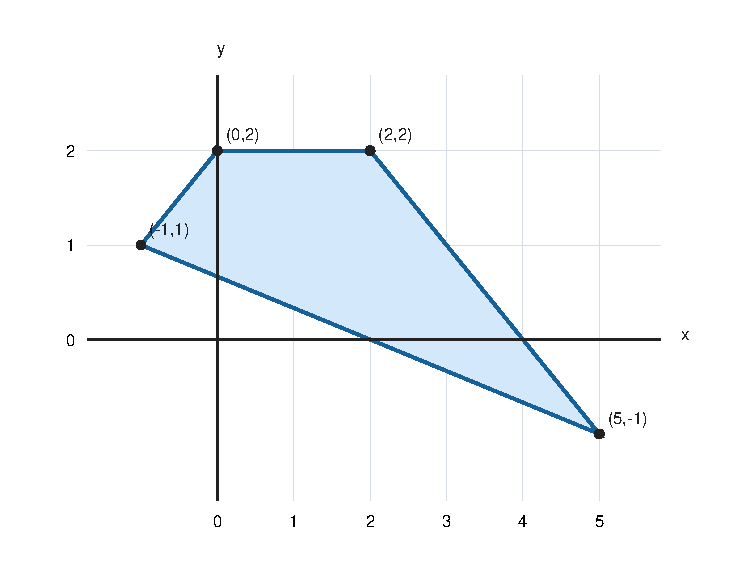
\includegraphics[width=0.49\linewidth]{recursos/figuras/s019-region.pdf}\end{center}

\textbf{b) Pertenencia del punto.}\par\nopagebreak[4]
Para $(4,-0.75)$, la expresión $x+3y$ vale $4-2.25=1.75<2$. Por ello el punto queda fuera.

\textbf{c) Extremos.}\par\nopagebreak[4]
En los cuatro vértices, $F$ vale $0$, $2$, $4$ y $4$. El mínimo $\boxed{0}$ se alcanza únicamente en $\boxed{(-1,1)}$. La restricción $x+y\le4$ da una cota superior alcanzada en toda la arista que une $(2,2)$ y $(5,-1)$. El máximo es $\boxed{4}$ y sus puntos son
\[
\boxed{(x,4-x),\qquad 2\le x\le5}.
\]
